\documentclass[journal,12pt,twocolumn]{IEEEtran}

\usepackage{setspace}
\usepackage{gensymb}

\singlespacing


\usepackage[cmex10]{amsmath}

\usepackage{amsthm}

\usepackage{mathrsfs}
\usepackage{txfonts}
\usepackage{stfloats}
\usepackage{bm}
\usepackage{cite}
\usepackage{cases}
\usepackage{subfig}

\usepackage{longtable}
\usepackage{multirow}

\usepackage{enumitem}
\usepackage{mathtools}
\usepackage{steinmetz}
\usepackage{tikz}
\usepackage{circuitikz}
\usepackage{verbatim}
\usepackage{tfrupee}
\usepackage[breaklinks=true]{hyperref}
\usepackage{graphicx}
\usepackage{tkz-euclide}

\usetikzlibrary{calc,math}
\usepackage{listings}
    \usepackage{color}                                            %%
    \usepackage{array}                                            %%
    \usepackage{longtable}                                        %%
    \usepackage{calc}                                             %%
    \usepackage{multirow}                                         %%
    \usepackage{hhline}                                           %%
    \usepackage{ifthen}                                           %%
    \usepackage{lscape}     
\usepackage{multicol}
\usepackage{chngcntr}

\DeclareMathOperator*{\Res}{Res}

\renewcommand\thesection{\arabic{section}}
\renewcommand\thesubsection{\thesection.\arabic{subsection}}
\renewcommand\thesubsubsection{\thesubsection.\arabic{subsubsection}}

\renewcommand\thesectiondis{\arabic{section}}
\renewcommand\thesubsectiondis{\thesectiondis.\arabic{subsection}}
\renewcommand\thesubsubsectiondis{\thesubsectiondis.\arabic{subsubsection}}


\hyphenation{op-tical net-works semi-conduc-tor}
\def\inputGnumericTable{}                                 %%

\lstset{
%language=C,
frame=single, 
breaklines=true,
columns=fullflexible
}
\begin{document}


\newtheorem{theorem}{Theorem}[section]
\newtheorem{problem}{Problem}
\newtheorem{proposition}{Proposition}[section]
\newtheorem{lemma}{Lemma}[section]
\newtheorem{corollary}[theorem]{Corollary}
\newtheorem{example}{Example}[section]
\newtheorem{definition}[problem]{Definition}

\newcommand{\BEQA}{\begin{eqnarray}}
\newcommand{\EEQA}{\end{eqnarray}}
\newcommand{\define}{\stackrel{\triangle}{=}}
\bibliographystyle{IEEEtran}
\providecommand{\mbf}{\mathbf}
\providecommand{\pr}[1]{\ensuremath{\Pr\left(#1\right)}}
\providecommand{\qfunc}[1]{\ensuremath{Q\left(#1\right)}}
\providecommand{\sbrak}[1]{\ensuremath{{}\left[#1\right]}}
\providecommand{\lsbrak}[1]{\ensuremath{{}\left[#1\right.}}
\providecommand{\rsbrak}[1]{\ensuremath{{}\left.#1\right]}}
\providecommand{\brak}[1]{\ensuremath{\left(#1\right)}}
\providecommand{\lbrak}[1]{\ensuremath{\left(#1\right.}}
\providecommand{\rbrak}[1]{\ensuremath{\left.#1\right)}}
\providecommand{\cbrak}[1]{\ensuremath{\left\{#1\right\}}}
\providecommand{\lcbrak}[1]{\ensuremath{\left\{#1\right.}}
\providecommand{\rcbrak}[1]{\ensuremath{\left.#1\right\}}}
\theoremstyle{remark}
\newtheorem{rem}{Remark}
\newcommand{\sgn}{\mathop{\mathrm{sgn}}}
\providecommand{\abs}[1]{\vert#1\vert}
\providecommand{\res}[1]{\Res\displaylimits_{#1}} 
\providecommand{\norm}[1]{\Vert#1\rVert}
%\providecommand{\norm}[1]{\lVert#1\rVert}
\providecommand{\mtx}[1]{\mathbf{#1}}
\providecommand{\mean}[1]{E[ #1 ]}
\providecommand{\fourier}{\overset{\mathcal{F}}{ \rightleftharpoons}}
%\providecommand{\hilbert}{\overset{\mathcal{H}}{ \rightleftharpoons}}
\providecommand{\system}{\overset{\mathcal{H}}{ \longleftrightarrow}}
	%\newcommand{\solution}[2]{\textbf{Solution:}{#1}}
\newcommand{\solution}{\noindent \textbf{Solution: }}
\newcommand{\cosec}{\,\text{cosec}\,}
\providecommand{\dec}[2]{\ensuremath{\overset{#1}{\underset{#2}{\gtrless}}}}
\newcommand{\myvec}[1]{\ensuremath{\begin{pmatrix}#1\end{pmatrix}}}
\newcommand{\mydet}[1]{\ensuremath{\begin{vmatrix}#1\end{vmatrix}}}
\numberwithin{equation}{subsection}
\makeatletter
\@addtoreset{figure}{problem}
\makeatother
\let\StandardTheFigure\thefigure
\let\vec\mathbf
\renewcommand{\thefigure}{\theproblem}
\def\putbox#1#2#3{\makebox[0in][l]{\makebox[#1][l]{}\raisebox{\baselineskip}[0in][0in]{\raisebox{#2}[0in][0in]{#3}}}}
     \def\rightbox#1{\makebox[0in][r]{#1}}
     \def\centbox#1{\makebox[0in]{#1}}
     \def\topbox#1{\raisebox{-\baselineskip}[0in][0in]{#1}}
     \def\midbox#1{\raisebox{-0.5\baselineskip}[0in][0in]{#1}}
\vspace{3cm}
\title{ASSIGNMENT-2}
\author{SOWMYA BANDI}
\maketitle
\newpage
\bigskip
\renewcommand{\thefigure}{\theenumi}
\renewcommand{\thetable}{\theenumi}
Download all python codes from 
\begin{lstlisting}
https://github.com/Sowmyabandi99/Assignment_2/blob/main/assignment2.py
\end{lstlisting}
%
and latex-tikz codes from 
%
\begin{lstlisting}
https://github.com/Sowmyabandi99/Assignment_2/blob/main/main.tex
\end{lstlisting}
%
\section{Question No. 2.40}
Construct PLAN where $PL = 4, LA = 6.5, \angle P = 90 \degree, \angle A = 110 \degree$ and $\angle N = 85 \degree$.
%
\section{SOLUTION}
\begin{enumerate}
\item Let us assume vertices of given quadrilateral $PLAN$ as $\vec{P}$,$\vec{L}$,$\vec{A}$ and $\vec{N}$.
\item Let us generalize the given data:
\begin{align}
&\angle P=90\degree=\theta \label{eq1}
\\
&\angle A=110\degree=\alpha
\\
&\angle N= 85\degree=\gamma \label{eq2}
\\
&\angle E=180\degree-\angle L=\delta,
\\
&\norm{\vec{L}-\vec{P}} =4=a, \label{eq3}
\\
&\norm{\vec{A}-\vec{L}} =6.5=b,\label{eq4}
\\
&\vec{P}=\myvec{0\\0}, \vec{L}=\myvec{4\\0} \label{eq5}
\end{align}
\item Also, let us assume the other two sides as
\begin{align}
 &\norm{\vec{N}-\vec{A}}=c \label{eq6}
\\
&\norm{\vec{P}-\vec{N}}=\norm{\vec{N}}=d \quad(\because \vec{P}=0) \label{eq7}
\end{align}  
\item We know,sum of angles of a quadrilateral = 360\degree
\begin{align}
\angle P + \angle L +\angle A +\angle N &= 360\degree
\\
90 \degree + \angle L + 110 \degree + 85 \degree &= 360\degree
\\
\implies \angle L &= 75 \degree \label{eq8}
\end{align}
\begin{itemize}
\item Now sum of all the angles given and \eqref{eq7} is $360\degree$.So construction of given quadrilateral is \textbf{possible}.
\end{itemize}
\begin{lemma}
\label{lemma}
The coordinates of A and N can be written as follows:
\begin{align}
\vec{A}=\vec{L} +b \myvec{\cos E\\\sin E} \label{eq9}
\\
\vec{N}=\vec{P} +d \myvec{\cos P\\\sin P} \label{eq10}
\end{align}
\end{lemma}
\begin{proof}
\begin{itemize}
\item For finding coordinates of A:
\end{itemize}
The vector equation of line is given by:
\begin{align}
\vec{A} &= \vec{L} +\lambda \myvec{\cos E\\\sin E} 
\\
\implies\norm{\vec{A}-\vec{L}} &= \abs{\lambda}\times\norm{\myvec{\cos 105\degree\\\sin 105\degree}} 
\\
\implies\norm{\vec{A}-\vec{L}} &= \abs{\lambda}\times1
\end{align}
Using \eqref{eq4} we get:
\begin{align}
\implies \abs{\lambda}=b 
\end{align}
\begin{itemize}
\item For finding coordinates of N:
\end{itemize}
The vector equation of line is given by:
\begin{align}
\vec{N}&=\vec{P}+\mu \myvec{\cos P\\\sin P}=\mu \myvec{\cos P\\\sin P} \quad(\because \vec{P}=0) 
\\
\implies\norm{\vec{N}} &= \abs{\mu}\times\norm{\myvec{\cos 90\degree\\\sin 90\degree}} 
\\
\implies\norm{\vec{N}} &= \abs{\mu}\times1
\end{align}
Using \eqref{eq6} we get:
\begin{align}
\implies \abs{\mu}=d
\end{align}
\item Using inner products of vectors we get,
\begin{align}
\frac{(A-N)^\intercal(A-L)}{\norm{A-N}\times\norm{A-L}}=\cos A \label{eq11}
\\
\frac{(A-N)^\intercal(P-N)}{\norm{A-N}\times\norm{P-N}}=\cos N \label{eq12}
\end{align}
\item Now, dividing \eqref{eq11} and \eqref{eq12} we get:
\begin{align}
\frac{(A-N)^\intercal(A-L)}{(A-N)^\intercal(P-N)}\times\frac{\norm{P-N}}{\norm{A-L}}=\frac{\cos A}{\cos N} \\
\frac{(A-N)^\intercal(A-L)}{(A-N)^\intercal(P-N)}\times\frac{d}{b}=\frac{\cos A}{\cos N}
\\
\frac{A^\intercal A-A^\intercal L-N^\intercal A+N^\intercal L}{-A^\intercal N+N^\intercal N}= \frac{b}{d}\times\frac{\cos A}{\cos N}  \quad(\because \vec{P}=0) 
\end{align}
\begin{align}
Let \quad S=b\times\frac{\cos A}{\cos N} \label{eq13}
\end{align}
\begin{align}
\implies d=\frac{S(-A^\intercal N+N^\intercal N)}{A^\intercal A-A^\intercal L-N^\intercal A+N^\intercal L}
\end{align}
\end{proof}
\item Now using \eqref{eq5}, \eqref{eq9} and \eqref{eq13} and solving we get
\begin{align}
\implies d=6.47
\end{align}
\item Putting values of b and d in \eqref{eq9} and \eqref{eq10}
\begin{align}
\vec{A}&=\myvec{a\\0} +b \myvec{\cos E\\\sin E} 
\\
\implies\vec{A}&=\myvec{4\\0} +6.5 \myvec{\cos 105\degree\\\sin 105\degree} 
\\
\implies\vec{A}&=\myvec{2.31\\6.27}
\end{align}
\begin{align}
and \quad \vec{N}&=d \myvec{\cos P\\\sin P}
\\
\implies\vec{N}&=6.47 \myvec{\cos 90\degree\\\sin 90\degree}
\\
\implies\vec{N}&=\myvec{0\\6.47}
\end{align}
\item Now,the vertices of given Quadrilateral PLAN can be written as,
\begin{align}
\vec{P}=\myvec{0\\0},\vec{L} = \myvec{4\\0}, \vec{A}=\myvec{2.31\\6.27},\vec{N}=\myvec{0\\6.47}
\end{align}
\item On constructing the quadrilateral $PLAN$ we get:
\end{enumerate}
\numberwithin{figure}{section}
\begin{figure}[!ht]
\centering
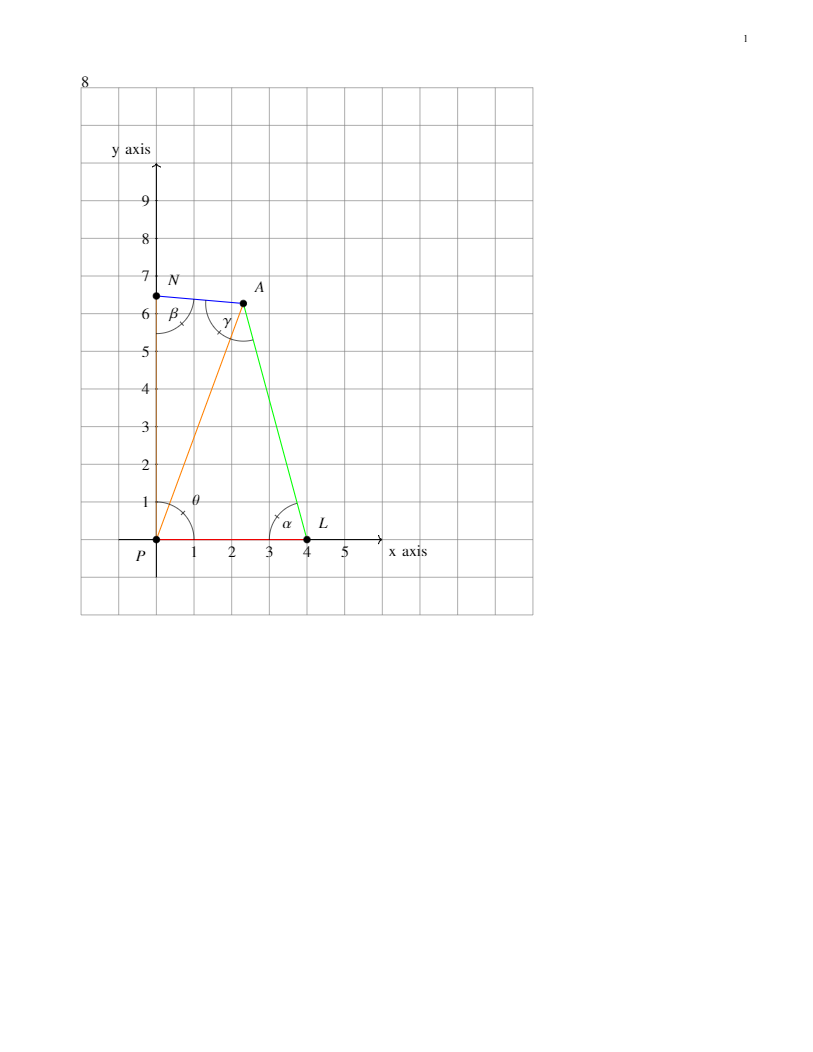
\includegraphics[height=20 cm]{Fig_PLAN.png}
\caption{Quadrilateral PLAN}
\end{figure}
\end{document}